\documentclass[11pt,a4paper]{report}
\usepackage[utf8]{inputenc}
\usepackage{amsmath}
\usepackage{amsfonts}
\usepackage{amssymb}
\usepackage{graphicx}
\usepackage{enumitem}
\usepackage[left=2cm, right=2cm, top=4.5cm, bottom=2cm]{geometry}

\begin{document}
	%Portada
	\begin{titlepage}
		\centering
		{\scshape\LARGE Universidad Nacional Autónoma de México \par}
		\vspace{1cm}
		{\scshape\Large Probabilidad I\par}
		\vspace{1.5cm}
		{\huge\bfseries Tarea VI\par}
		\vspace{.5cm}

		{\Large\itshape Alan Ernesto Arteaga Vázquez \par}
		 \vspace{.5cm}
		{\Large\itshape Raúl Llamosas Alvarado \par}
		 \vspace{.5cm}
		{\Large\itshape Edgar Quiroz Castañeda \par}
	    \vspace{.5cm}
		{\Large\itshape Jean Paul Ruiz Melo\par}
		\vspace{.5cm}
		{\Large\itshape Sandra Del Mar Soto Corderi \par}

		\vfill
		 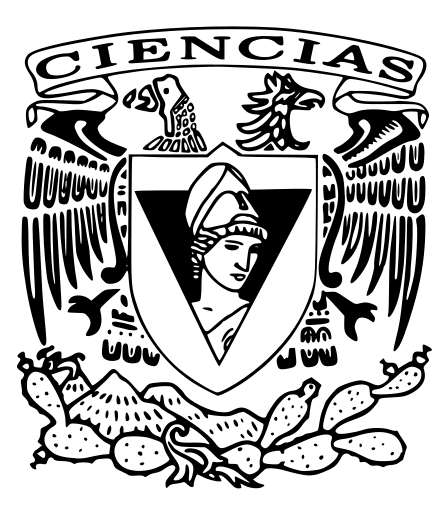
\includegraphics[width=0.3\textwidth]{escudo.png}
		\vfill

		{\large Martes 20 de noviembre del 2018 \par}
	\end{titlepage}

	\pagebreak
	\setlength{\voffset}{-0.75in}
	\setlength{\headsep}{5pt}

	%Ejericios
	\begin{enumerate}
		%1
		\item{
			Sea $X\sim\text{Poisson}(\lambda)$, demuestre que
            \[F_X(n) = \frac{1}{n!}\int_{\lambda}^{\infty}e^{-x}x^n dx\]
			Resolviendo la integral por partes, tenemos que
			\[\int_{\lambda}^{\infty}e^{-x}x^n dx
			= -e^{-x}x^n \Big|_{\lambda}^{\infty}+
			n\int_{\lambda}^{\infty}{e^{-x}x^{n-1}dx}
			= e^{-\lambda}\lambda^n + n\int_{\lambda}^{\infty}{e^{-x}x^{n-1}dx}\]
			Repitiendo este proceso $n$ veces, tenemos que la integral es de la
			forma
			\begin{align*}
				\int_{\lambda}^{\infty}e^{-x}x^n dx
				&= e^{-\lambda}\lambda^n + n(e^{-\lambda}\lambda^{n-1} +
				(n-1)(e^{-\lambda}\lambda^{n-2} + \dots + 2(e^{-\lambda}\lambda +
				e^{-\lambda})\dots))\\
				&= e^{-\lambda}\lambda^n + ne^{-\lambda}\lambda^{n-1} +
				n(n-1)e^{-\lambda}\lambda^{n-2} + \dots
				+ n(n-1)\dots(2)e^{-\lambda}\lambda + n!e^{-\lambda}
			\end{align*}
			Entonces
			\begin{align*}
				\frac{1}{n!}\int_{\lambda}^{\infty}e^{-x}x^n dx
				&= \frac{1}{n!}(e^{-\lambda}\lambda^n + ne^{-\lambda}\lambda^{n-1} +
				n(n-1)e^{-\lambda}\lambda^{n-2} + \dots n!e^{-\lambda} )\\
				&= \frac{e^{-\lambda}\lambda^n}{n!} + \frac{ne^{-\lambda}\lambda^{n-1}}{n!}
				+ \frac{n(n-1)e^{-\lambda}\lambda^{n-2}}{n!} + \dots +
				\frac{n!e^{-\lambda}}{n!}\\
				&= \frac{e^{-\lambda}\lambda^n}{n!} +
				\frac{e^{-\lambda}\lambda^{n-1}}{(n-1)!} +
				\frac{e^{-\lambda}\lambda^{n-2}}{(n-2)!} + \dots +
				e^{-\lambda}\lambda + e^{-\lambda}
			\end{align*}
			Por otra parte, como $X\sim\text{Poisson}(\lambda)$, entonces
			su densidad es
			\[f_X(n) = \frac{e^{-\lambda}\lambda^{n}}{n!}\]
			con $x = \{0, 1, 2, 3, ...\}$.\\
			Luego, por definición de distribución,
			\[F_X(n) = \sum_{i=0}^{n}{\frac{e^{-\lambda}\lambda^{i}}{i!}}
			= e^{-\lambda} + e^{-\lambda}\lambda^{1} + \frac{e^{-\lambda}\lambda^{2}}{2}
			+ \dots  + \frac{e^{-\lambda}\lambda^{n-1}}{(n-1)!} +
			\frac{e^{-\lambda}\lambda^n}{n!}\]
			Que es exactamente la expansión de la integral. Por lo tanto,
			\[F_X(n) = \frac{1}{n!}\int_{\lambda}^{\infty}e^{-x}x^n dx\]
		}

		%2
		\item{
			Suponga que en un grupo de probabilidad de 100 alumnos, el 85\% de
            los alumnos reprobó el segundo examen parcial. Si tomamos una
            muestra de tamaño 30. Calcule la probabilidad de
            \begin{enumerate}
                %a
                \item {
                	Exactamente 10 alumnos de la muestra hayan reprobado.\\
					Esto implicaría que 20 alumnos de la muestra aprobaron,
					lo cuál es imposible pues sólo 15 aprobaron.
					Entonces la probabilidad de que eso pase es 0.
                }

                %b
                \item {
                	Al menos 5 alumnos de la muestra hayan reprobado.\\
					Como sólo 15 aprobaron, entonces al menos 15 reprobaron.
					En particular, siempre se tiene que al menos 5 aprobaron.
					Entonces eso probabilidad es 1.
                }

                %c
                \item {
                	El número de alumnos reprobados de la muestra esté entre 5 y 10.\\
					Hay al menos 15 alumnos reprobados. Entonces, nunca hay entre
					5 y 20 reprobados. Entonces, la probabilidad de eso es 0.
                }
            \end{enumerate}
		}

		%3
		\item{
            Una aseguradora tiene 10 pólizas independientes con una cobertura
            de una año. El valor nominal de cada una de esas pólizas es de
            \$1,000. La probabilidad de que haya una reclamación en el año en
            consideración es de 0.1. Encuentre la probabilidad de que la
            aseguradora pague más del total esperado para el año en
            consideración.\\
			Sea $X$ la variable aleatoria que representa el número de polizas
			a pagar en el año. Tenemos que cada póliza es independiente de las
			demás, y cada una tiene probabilidad de 0.1 de ser pagada.\\
			Entonces, si consideramos que el pagar una poliza es un éxito,
			tenemos que $X \sim  Bin(0.1, 10)$, por lo que
			\[f_X(x) = {10 \choose x}(0.1)^x (0.9)^{10-x}\]
			Y la esperanza, o sea el número esperado de pólizas a pagar, es
			\[E(X) = np = 10 \times 0.1 = 1\]
			Por lo que se espera pagar una póliza, es decir \$1000.\\
			Entonces se busca
			\[P(X > 1) = 1 - P(X \leq 1) = 1 - P(X = 0) - P(X = 1) = 1 - f_X(0) - f_X(1)\]
			Tenemos que
			\begin{align*}
				&f_X(0) = {10 \choose 0}(0.1)^0 (0.9)^{10} = (0.9)^{10} \approx 0.35 \\
				&f_X(1) = {10 \choose 1}(0.1)^1 (0.9)^9 = 0.1 \cdot (0.9)^9 \approx 0.04\\
				&\implies P(X > 1) = 1 - (0.9)^{10} - 0.1 \cdot (0.9)^9 \approx 0.61
			\end{align*}
			Entonces, hay una probabilidad de más o menos $61\%$ de que la
			aseguradora pague más de lo esperado.
		}

		%4
		\item{
			Una moneda es lanzada tantas veces como sea necesario hasta obtener
            5 águilas. Si se sabe que en los primeros 8 lanzamientos no se ha
            logrado el objetivo. Calcule la probabilidad de que se requieran, en
            total, menos de 12 lanzamientos.\\
			Se busca la probabilidad de que se logre obtener las 5 águilas en 9,
			10 u 11 lanzamientos, dado que no se han obtenido las 5 águilas en
			los 8 primero lanzamientos. Es decir, la probabilidad de obtener a
			los más 6 fracasos antes del quinto éxito dado que han ocurrido
			al menos 4 fracasos. \\
			Esto es una distribución binomial negativa.\\
			Es decir $X \sim BinNeg(\frac{1}{2}, 5)$. Esto significa que
			\[f_X(x) = {x+5-1 \choose x} \frac{1}{2}^5 \frac{1}{2}^x =
			{x+5-1 \choose x} \frac{1}{2}^{5+x}\]
			Como estas probabilidades son independientes entonces la probabilidad
			de que ocurra alguna de ellas es la suma de las probabilidades.
			\[f_X(0) = {4 \choose 0} \frac{1}{2}^{5} = \frac{1}{32}\]
			\[f_X(1) = {5 \choose 1} \frac{1}{2}^{6} = \frac{5}{64}\]
			\[f_X(2) = {6 \choose 2} \frac{1}{2}^{7} = \frac{15}{128}\]
			\[f_X(3) = {7 \choose 3} \frac{1}{2}^{8} = \frac{35}{256}\]
			\[f_X(4) = {8 \choose 4} \frac{1}{2}^{9} = \frac{70}{512}\]
			\[f_X(5) = {9 \choose 5} \frac{1}{2}^{10} = \frac{126}{1024}\]
			\[f_X(6) = {10 \choose 6} \frac{1}{2}^{11} = \frac{210}{2048}\]
			\begin{align*}
				P(X \leq 6 | X \geq 4) &= \frac{P(X \leq 6 \cap X \geq 4)}{P(X \geq 4)}\\
							  &=\frac{P(X \leq 6 \cap X \geq 4)}{1-P(X < 4)}  \\
							  &=\frac{f_X(4) + f_X(5) + f_X(6)}
							  {1-(f_X(0) + f_X(1) + f_X(2)+ f_X(3))}  \\
							  &= \frac{\frac{140+126+105}{1024}}
							  {1-\frac{8+20+30+35}{256}} \\
							  &= \frac{\frac{371}{1024}}{1-\frac{93}{256}} \\
							  &= \frac{\frac{371}{1024}}{\frac{163}{256}} \\
							  &= \frac{371}{652} \\
							  &\approx 0.57
			\end{align*}
		}

		%5
		\item{
			Un dado balanceado es lanzado hasta que cae la cara con el "4". Si X
            es el número de lanzamientos requeridos hasta obtener el primer "4".
            ¿Cuál es el valor de $\epsilon$ más pequeño para el cual
            $P(X \leq \epsilon) \geq 0.5$?\\
            Tenemos que éste problema describe una variable aleatoria con distribución geométrica. La cual está dada por:
            $$p(i)=p(1-p)^{i-1}: i\in \lbrace 1,2,... \rbrace $$
            Que un dado caiga con una cara "x" tiene probabilidad de $\frac{1}{6}$ entonces en éste caso $p=\frac{1}{6}$, $1-p=\frac{5}{6}$. Tenemos que $P(X\leq \epsilon) $ es una función de distribución de una variable discreta que está dada por:
            $$P(X\leq \epsilon)=F(\epsilon)=\sum_{i=0}^{\epsilon}p(i)=\sum_{i=0}^{\epsilon}(\frac{1}{6})(\frac{5}{6})^{i-1}=\sum_{i=0}^{\epsilon}(\frac{5^{i-1}}{6^{i}})=\frac{1}{5}\sum_{i=0}^{\epsilon}(\frac{5}{6})^{i}=\frac{1}{5}(\frac{(\frac{5}{6})^{\epsilon+1}-1}{\frac{5}{6}-1})$$ Y esto es mayor a $\frac{1}{2}$ cuando:
            $$\frac{1}{5}(\frac{(\frac{5}{6})^{\epsilon+1}-1}{-\frac{1}{6}})\geq \frac{1}{2}\Leftrightarrow \frac{1}{5}((\frac{5}{6})^{\epsilon+1}-1)\leq -\frac{1}{12}$$
            $$(\frac{5}{6})^{\epsilon+1}\leq -\frac{5}{12}+1=\frac{7}{12}$$
            $$(\frac{5}{6})^{\epsilon+1}\leq \frac{7}{12}$$

            Tenemos que la igualdad se da cuando:
            $$(\frac{5}{6})^{\epsilon+1}=\frac{7}{12}\Leftrightarrow log_{\frac{5}{6}}(\frac{7}{12})=\epsilon+1 \Leftrightarrow \epsilon=log_{\frac{5}{6}}(\frac{7}{12})-1
            $$
            Por propiedades de logaritmo esto es igual a:
            $$\epsilon=log_{\frac{5}{6}}(\frac{7}{12})-1=log_{\frac{5}{6}}(7)-log_{\frac{5}{6}}(12)-1=\frac{ln(7)-ln(12)-ln(\frac{5}{6})}{ln(\frac{5}{6})}=\frac{ln(7)-ln(2)-ln(5)}{ln(5)-ln(2)-ln(3)}$$
            Por desigualdades de logaritmo. Se sigue entonces que:
            $$(\frac{5}{6})^{\epsilon+1}\leq \frac{7}{12}\Leftrightarrow e\geq \frac{ln(7)-ln(2)-ln(5)}{ln(5)-ln(2)-ln(3)}_{\blacksquare}$$
		}

		%6
		\item{
			En una tienda de abarrotes se venden 400 artículos, 6 de los cuales
            no tienen marcada la clave de su precio. Si una persona entra a la
            tienda y elige 10 artículos, calcule la probabilidad de que entre
            los  artículos escogidos haya por lo menos un artículo que no tenga
            marcada la cave de su precio.
            \\
            Usamos la distribución hipergeométrica. Tenemos entonces que ésta está dada por:
            $$p(i)=\frac{\binom{m}{i}\binom{N-m}{n-i}}{\binom{N}{n}}$$
            Y se tiene que en éste caso N=400,n=10,m=6,i=1. Entonces se sigue que:

            $$p(1)=\frac{\binom{6}{1}\binom{400-6}{10-1}}{\binom{400}{10}}\approx 0.1337 $$
		}

		%7
		\item{
			Supongamos que el 5\% de las personas mayores de 18 años tiene su
            INE vencida. Utilice la aproximación Poisson para estimar la
            probabilidad de que a lo más 3 de 50 personas mayores de 18 años,
            seleccionadas al azar, tengan su INE vencida.\\
            La probabilidad de Poisson dice que:
            $$P\lbrace X=i \rbrace = e^{-\lambda} \frac{\lambda^{i}}{i!}$$
            Tenemos que 3 de 50 personas da una relación de $\frac{3}{50}=0.06 \rightarrow 6\%$. 5 de cada 100 personas mayores a 18 años tienen su INE vencida entonces $\lambda=5$. Entonces la probabilidad de que 6 de cada 100 tenga su INE vencida está dada por
            $$P(6 \ INE \ vencidas \ cada \ 100)=\frac{\lambda^{k}e^{-\lambda}}{k!}=\frac{5^{6}e^{-6}}{6!}=\frac{15625}{e^{6} 6!}\approx 0.05379$$
		}

		%8
		\item{
			\begin{enumerate}
				%a
				\item {
					Encuentre la moda de la distribución gamma.


				Tenemos que la función de distribución gamma con parámetros $\lambda$ y $\omega$ está dada por
				$$f(x)=\frac{\lambda e^{-\lambda x}(\lambda x)^{\omega-1}}{\Gamma(\omega)}=\frac{\lambda e^{-\lambda x}(\lambda x)^{\omega -1}}{\int_{0}^{\infty}e^{-x}x^{\omega -1}dx}$$ Y la moda se define como el valor $x_{m}$ tal que $$f'(x_{m})=0$$
				Es decir cuando alcance un máximo. Hagamos la siguiente afirmación:\\
				\textbf{Afirmación:} $\Gamma(\omega)=(\omega-1)!$ \\
				\textit{Demostración:} Tomemos como caso base $\Gamma(1)$ tenemos que $$\Gamma(1)=\int_{0}^{\infty}e^{-x}x^{1-1}dx=\int_{0}^{\infty}e^{-x}dx=[-e^{-x}]_{0}^{\infty}=\lim_{x\rightarrow \infty}(-e^{-x})+e^{-0}=1$$
				Ahora supongamos que para $n$ se cumple $\Gamma(n)=(n-1)!$. Demostremos que para $\Gamma(n+1)$ se cumple que $\Gamma(n+1)=n!$. Tenemos que: $$\Gamma(n+1)=\int_{0}^{\infty}e^{-x}x^{n+1-1}dx=\int_{0}^{\infty}e^{-x}x^{n}dx$$ Utilizando integración por partes uno puede ver que es igual a $$=[-x^{n}e^{-x}]_{0}^{\infty}+\int_{0}^{\infty}n  x^{n-1}e^{-x}dx=\lim_{x\rightarrow \infty}(-x^n e^{-x})-(-0^{n} e^{-0})+n\int_{0}^{\infty}x^{n-1}e^{-x}dx$$ $$=n\int_{0}^{\infty}x^{n-1}e^{-x}dx=n\Gamma(n)$$
				Y esto resulta de conocer previamente que $\lim_{x \rightarrow \infty}(-x^{n}e^{-x})=0$. Además, como por hipótesis de inducción tenemos que $\Gamma(n)=(n-1)!$ se sigue que $$n\Gamma(n)=n(n-1)!=n!_{\blacktriangle}$$ Entonces, tenemos que $$f(x)=\frac{\lambda e^{-\lambda x}(\lambda x)^{\omega-1}}{(\omega-1)!}=\frac{(\lambda)^{\omega}e^{-\lambda x}x^{\omega-1}}{(\omega-1)!}=\frac{\lambda^{\omega}}{(\omega-1)!}(e^{-\lambda x}x^{\omega-1})$$ Tenemos entonces que la derivada estará dada por $$f'(x)=(\frac{\lambda^{\omega}}{(\omega-1)!}) (-\lambda e^{-\lambda x}x^{\omega-1}+(\omega-1)x^{\omega-2}e^{-\lambda x})$$ Y se hace cero cuando $$ -\lambda e^{-\lambda x}x^{\omega-1}+(\omega-1)x^{\omega-2}e^{-\lambda x}=0$$ $$(\omega-1)x^{\omega-2} e^{-\lambda x}=\lambda e^{-\lambda x}x^{\omega-1}$$ $$(\omega-1)=\lambda (\frac{e^{-\lambda x} x^{\omega-1}}{e^{-\lambda x}x^{\omega-2}})$$ $$(\omega-1)=\lambda x$$ $$x=\frac{\omega-1}{\lambda}$$
	Tenemos además que la segunda derivada está dada por:
				$$f''(x)=(\frac{\lambda^{\omega}}{(\omega-1)!})(\lambda^2 e^{-\lambda x}x^{\omega-1}-\lambda(\omega-1)x^{\omega-2}e^{-\lambda x}+(\omega-1)((\omega-2)x^{\omega-3}e^{-\lambda x}-\lambda(\omega-1)e^{-\lambda x})$$
				Tenemos que $f''(\frac{\omega-1}{\lambda})<0$ entonces se trata de un máximo por lo tanto se concluye que la moda es $x_{m}=\frac{\omega-1}{\lambda}_{\blacksquare}$
				Entonces se concluye que la moda es $x_{m}=\frac{\omega-1}{\lambda}_{\blacksquare}$
				}

				%b
				\item {
					Si $X \sim \text{exp}(\lambda)$, demuestre que
                        $$ \mathbb{E}(X^k) = \frac{k!}{\lambda^k} $$

                        Se dice que $X \sim \text{exp}(\lambda)$ si su funcion de densidad es de la forma $$f(x)= 	\begin{cases}
		\lambda e^{-\lambda x} \ si \ x\geq 0 \\
		0 \ si \ x<0
	\end{cases}$$ Tenemos que la función generadora de momentos está dada por: $$E(e^{tx})=\int_{0}^{\infty}e^{tx}(\lambda e^{-\lambda x}) dx=\lambda \int_{0}^{\infty}e^{x(t-\lambda)}dx=\lambda ([\frac{e^{x(t-\lambda)}}{t-\lambda}]_{0}^{\infty})=\lambda (\lim_{x\rightarrow \infty} (\frac{e^{x(t-\lambda)}}{t-\lambda})-\frac{e^{0(t-\lambda)}}{t-\lambda})=\frac{\lambda}{\lambda-t}$$
	Donde la función generadora denotada por $M_{x}(t)$ es una función con variable t.La propiedad que cumple la función generadora de momentos es que $$E(X^{k})=\lim_{t\rightarrow 0}( (\frac{d^{k}}{dx^{k}}) E(e^{tx}))$$ Es decir
	$$E(X^{k})=\lim_{t\rightarrow 0}(\frac{\lambda}{\lambda-t})^{(k)}$$ Usando la notación de Lagrange para denotar la k-ésima derivada. \\
	\textbf{Afirmación:} $M_{x}(t)^{(k)}=\frac{\lambda k!}{(\lambda-t)^{k+1}}$. \\
	\textit{Demostración:}Procedemos por inducción sobre el número de derivadas de la función generadora de momentos $\frac{\lambda}{\lambda-t}$. Tomamos caso base k=1, es decir la primera derivada:
	$$M_{x}(t)^{(1)}=(\frac{\lambda}{\lambda-t})^{(1)}=\frac{\lambda 1!}{(\lambda-t)^2}$$ Ahora suponemos que la n-ésima derivada de la función está dada por $M_{x}(t)^{(n)}=\frac{\lambda(n!)}{(\lambda-t)^{n+1}}$ tomemos entonces:
	$$M_{x}(t)^{(n+1)}=(M_{x}(t)^{(n)})^{(1)}=(\frac{\lambda (n!)}{(\lambda-t)^{n+1}})^{(1)}=\frac{\lambda (n+1)(n!)}{(\lambda-t)^{n+2}}=\frac{\lambda (n+1)!}{(\lambda-t)^{n+2}}$$ Entonces la afirmación es correcta. Entonces, tenemos que $$E(X^{k})=\lim_{t\rightarrow 0}(M_{x}(t))^{(k)}=\lim_{t \rightarrow 0}(\frac{\lambda(k!)}{(\lambda-t)^{k+1}})=\frac{\lambda k!}{\lambda^{k+1}}=\frac{k!}{\lambda^{k}}_{\blacksquare}$$
				}

			\end{enumerate}
		}

			%9
		\item{
			Sea X una variable aleatoria continua con función de distribución F.
            Defínase Y una variable aleatoria tal que $Y = F(X)$. Demuestre que
            $Y \sim \text{Unif}(0,1)$.
            \\
            Primero tenemos:
            \[F(y) = y\]
            De donde:
            \[y = F(x)\]
            Entonces:
            \[F_{x}(y) = \mathbb{P}(Y \leq y) = \mathbb{P}(F(x) \leq y)\]
            Entonces, esto es igual a:
            \[\mathbb{P}(F(x) \leq y) = \mathbb{P}(X \leq F^{-1}(y)) = y\]
            Y el unico distribucion que tiene este forma es $Y \sim \text{Unif}(0,1)$.


		}

		%10
		\item{
			Conteste las siguientes preguntas respecto a la distribución normal.
			\begin{enumerate}
				%a
				\item {
					Demuestre que la función de densidad $N(\mu, \sigma^2)$ es
                    simétrica con respecto a $x = \mu$, alcanza su máximo en
                    $x = \mu$ y tiene puntos de inflexión en $x_1= \mu + \sigma$
                    y $x_2 = \mu - \sigma$.\\
				}

				%b
				\item {
					Si X es una variable aleatoria con distribución normal con
                    parámetros $\mu = 10$ y $\sigma^2 = 36$.\\
                    Calcule: $\mathbb{P}(X > 5)$, $\mathbb{P}(4 < X < 10)$,
                    $\mathbb{P}(X < 8)$, $\mathbb{P}(X < 20)$ y
                    $\mathbb{P}(X > 16)$.\\

                    Tenemos  $N(\mu = 10, \sigma^2 = 36)$, de donde $\sigma = 6$.
                    Entonces:
                    \[ \mathbb{P}(X > 5) = 1 - \mathbb{P}(z \leq \frac{5-10}{6}) =1 - (1 -  F_z(\frac{5}{6})) =  Fz(0.83) = 0.7967 \]

                    \[ \mathbb{P}(4 < x < 10) = \mathbb{P}(\frac{4-10}{6} < z < \frac{10-10}{6}) =\mathbb{P}(-1 < z < 0) =  F_z(0) - (1 - F_z(1))\]
                    \[= 0.5 - 1 + 0.8413 = 0.3413 \]

                    \[ \mathbb{P}(X < 8) = \mathbb{P}(z < \frac{8-10}{6}) = F_z(-\frac{1}{3}) = 1 - F_z(0.33) = 1 - 0.6293 = 0.3707 \]

                     \[ \mathbb{P}(X < 20) = \mathbb{P}(z < \frac{20-10}{6}) = F_z(\frac{10}{6}) = F_z(1.66) = 0.9515 \]

                     \[ \mathbb{P}(X > 16) = 1 - \mathbb{P}(z \leq \frac{16-10}{6}) = 1 -  F_z(1) =  1 - 0.8413 = 0.1587 \]
				}

				%c
				\item {
				Suponga que X es una variable aleatoria con distribución normal con media 5 .$\mathbb{P} (X > 9) = \frac{1}{5}$, calcule la varianza de X.\\

				Tenemos que:
				\[\mathbb{P}(X > 9) = 1 - \mathbb{P}(X \leq 9) = .20\]
				Entonces:
				\[- \mathbb{P}(X \leq 9) = - 0.80\]
				\[\mathbb{P}(X \leq 9) = 0.80 \]
				Queremos encuentrar $\sigma$, entonces:
				\[\phi(\frac{9 - 5}{\sigma}) = 0.80 \]
				\[\phi(\frac{4}{\sigma}) = 0.80\]
				En la tabla, $0.80$ esta dentro de $\phi(.84)$ y $\phi(.85)$ tal que:
				\[\phi(.84) < 0.80 < \phi(.85) \]
				\[.7945 < .80 < .8023\]
				Aplicando la integral con $0.845$ se acerca a .80 por 2 decimales con 0.8009, entonces para:
				\[\mathbb{P}(X \leq 9) = \phi(\frac{4}{\sigma}) \approx \phi(0.845)\]
				Resolviendo $\frac{4}{\sigma} \approx 0.845$ para $\sigma$ se tiene:
				\[ \sigma \approx \frac{4}{0.845} = 4.73\]
				Por lo tanto:
				\[ \sigma \approx 4.73 ; \sigma^2 \approx 22.40 \]
				Entonces la varianza de X es aproximadamente 22.4.
				}

				%d
				\item {
					Sea $X$ una variable aleatoria con distribución normal con
					media 12 y varianza 4. Encontrar el valor de $\tau$ tal que
					$\mathbb{P}(X < \tau) \in \{0,1\}$.\\
					Tenemos que cuando x de $\phi(x)$ es igual a infinito, da 1. Y que cuando x es igual a menos infinito, da 0. Entonces:
					\[\phi(-\infty) \leq \frac{r-\mu}{\sigma} \leq \phi(\infty)\]
					Para esto tenemos:
					\[\frac{r-\mu}{\sigma} = -\infty\]
					\[ r - \mu = -\infty \sigma = -\infty\]
					\[r = -\infty - \mu \]
					\[r = -\infty\]
					Lo cual seria analogamente con $\infty$. Por lo tanto r puede tener valor de:
					\[ -\infty \leq r \leq \infty \]
					Ya que:
					\[\int^{\infty}_{-\infty}\frac{1}{\sigma\sqrt{2\pi}}e^{\frac{1}{2}(\frac{x-\mu}{\sigma})^2} = 1\]
				}

				%e
				\item {
					Si $X$ tiene una distribución normal con media $\mu = 9$ y
					varianza $\sigma^2 = 4$, encontrar \\
					$\mathbb{P}(X^2 - 2X \leq 8)$\\
					Tenemos $\mathbb{P}(X^2 - 2X \leq 8)$, resolviendo para X tenemos:
					\[X^2 - 2X - 8 = 0\]
					\[(X + 2) (X - 4) = 0\]
					Entonces:
					\[\mathbb{P}(-2 < X < 4) \]
					De donde:
					\[ \mathbb{P}(-2 < x < 4) = \mathbb{P}(\frac{-2-9}{2} < z < \frac{4-9}{2}) =\mathbb{P}(\frac{-11}{2} < z < \frac{-5}{2}) =  (1 - F_z(2.5)) - (1 - F_z(5.5))\]
					\[  1 - \phi(2.5) = 1 - 0.9938 = 0.0062\]
					\[ 1 - \phi(5.5) = 1 - 0.9999 = 0.0001 \]
					\[\mathbb{P}(-2 < x < 4) = 0.0062 - 0.0001 = 0.0061\]
				}
			\end{enumerate}
		}

		%11
		\item{
			Sea $X$ una variable aleatoria con distribución uniforme en el
			intervalo $(-\frac{\pi}{2}, \frac{\pi}{2})$. Encuentre la función de
			distribución y la función de densidad $Y = \tan(X)$.\\
			\[FY(y) = P(Y = y)\]
		\[=P(tan(X) \le y\]
		Si resolvemos para y:
		\[P(X \le arctan(y))\]
		\[Fx(arctan(y))\]
		\[= \int^{arctan(y)}_{-\frac{\pi}{2}}\frac{1}{\frac{\pi}{2}- (- \frac{\pi}{2}}dx\]
		\[= \int^{arctan(y)}_{-\frac{\pi}{2}} \frac{1}{\pi}\]
		\[=\frac{1}{\pi}|^{arctan(y)}_{-\frac{\pi}{2}}\]
		\[FY(y)=\frac{arctan(y) + \frac{\pi}{2}}{2}\]

		}

		%12
		\item{
			Si $X \sim \text{Unif}(0, 10)$, calcular
			$\mathbb{P}(X + \frac{10}{X} > 7)$\\
			Resolviendo para X tenemos:
			\[X + \frac{10}{X} - 7 = 0\]
			\[ (x - 5) (x - 2) = 0\]
			De donde se tiene:
			\[x_1 = 5 ; x_2 = 2\]
			\[\mathbb{P}(0 < x < 2) + \mathbb{P}(5 < x <10)\]
			Calculando tenemos:
			\[\int^{2}_{0}\frac{1}{10-0}dx + \int^{10}_{5}\frac{1}{10-0}dx = \frac{1}{5} + \frac{1}{2} = \frac{7}{10}\]

		}


		%13
		\item{
			Un aparato mide y graba de manera continua la actividad sísmica de
			una región remota. El tiempo, $T$, de falla del aparato se
			distribuye exponencial con media de 3 años. Debido a que el aparato
			no será monitoreado durante sus dos primeros años de servicio, el
			tiempo para descubrir una falla es $X = \text{máx}\{T,2\}$.
			Encuentre $\mathbb{E}(X)$.

			Se tiene, como T se distribuye exponencial con media de 3 años:
				$$ T \sim Exp(\lambda), f_T^{(t)} = \lambda e^{-\lambda t}$$
			y se cumple:
				$$ \mathbb{E}(T) = \frac{1}{\lambda}$$
			como se supone una media de 3 años:
				$$ 3 = \frac{1}{\lambda} \Rightarrow \lambda = \frac{1}{3}$$
			se tiene $g(T) = X = max\{T, 2\}$, para hallar $\mathbb{E}(X)$,
			usando la "Ley del estadístico inconsciente":
				$$ \mathbb{E}[g(T)] = \int_{-\infty}^{\infty} g(T) f_T{(t)}dt $$
				$$ \mathbb{E}[max\{T,2\}] = \int_{-\infty}^{\infty} max\{T,2\}
				 							\lambda e^{-\lambda t} dt $$
			como $T \sim Exp(\lambda)$, se tiene $t > 0$, así:
				$$ \mathbb{E}[max\{T,2\}] = \lambda \int_{0}^{\infty} max\{T,2\}
				 							e^{-\lambda t} dt $$
			Como $max\{T,2\} = t$ si $t \geq 2$ y $max\{T,2\} = 2$ si $t < 2$,
			entonces:
				$$ \mathbb{E}[X] =\lambda \Big[ 2\int_{0}^{2} e^{-\lambda t} dt
				              + \int_{2}^{\infty} t e^{-\lambda t} dt \Big] $$
				$$ \mathbb{E}[X] =\lambda \Big[ 2 \cdot
								 \frac{1}{-\lambda}\int_{u(0)}^{u(2)} e^u du
				              + \int_{2}^{\infty} t e^{-\lambda t} dt \Big] $$
				$$ \mathbb{E}[X] =\lambda \Big[
								 \frac{2}{-\lambda} \Big[ e^{-\lambda t}
								 \Big]_{t=0}^{2}
				              + \int_{2}^{\infty} t e^{-\lambda t} dt \Big]
							  	...(A)$$

			integrando por partes $\int_{2}^{\infty} t e^{-\lambda t} dt$, se
			tiene, considerando $u = t$, $dv = e^{-\lambda t} $
				$$ \int_{2}^{\infty} t e^{-\lambda t} dt
				=  \Big[ t \frac{1}{- \lambda} e^{-\lambda t} \Big]_{2}^{\infty}
					- \int_{2}^{\infty} \frac{1}{- \lambda} e^{-\lambda t} dt$$
				$$ = \frac{\infty \cdot e^{-\infty}}{-\lambda}
				   + \frac{2e^{-2\lambda}}{\lambda} + \frac{1}{\lambda}
				    \Big[ \frac{1}{- \lambda } (e^{-\lambda
					t})_{0}^{\infty}\Big]$$
				$$ = \frac{\infty \cdot e^{-\infty}}{-\lambda}
				   + \frac{2e^{-2\lambda}}{\lambda} + \frac{1}{\lambda}
				    \Big[ \frac{1}{\lambda } (e^{-2 \lambda})\Big]$$
				$$ = 0 + \frac{2e^{-2\lambda}}{\lambda}
				   + \frac{ e^{-2 \lambda} }{\lambda^2} $$
			De (A), se tiene:
				$$ \mathbb{E}[X] =\lambda \Big[
								 \frac{2}{-\lambda} \Big[ e^{-\lambda t}
								 \Big]_{t=0}^{2}
							  + \int_{2}^{\infty} t e^{-\lambda t} dt \Big]
					= \lambda \Big[ \frac{2e^{-2\lambda}}{-\lambda}
								  +	\frac{2}{\lambda}
								  + \frac{2e^{-2\lambda}}{\lambda}
								  + \frac{ e^{-2 \lambda} }{\lambda^2} \Big]$$
				$$ = \lambda \Big[ \frac{2}{\lambda}
							     + \frac{ e^{-2 \lambda} }{\lambda^2} \Big]
				   = 2 + \frac{ e^{-2 \lambda} }{\lambda}
				   = 2 + \frac{ e^{- \frac{2}{3}} }{\frac{1}{3}}
				   = 2 + 3e^{-\frac{2}{3}} $$
			Concluimos así, para la variable aleatoria $X$:
				$$ \mathbb{E}[X] = 2 + 3e^{-\frac{2}{3}} $$

		}

		%14
		\item{
			Demuestre que si $X \sim \text{Hipergeométrica}(N,m,n)$, entonces.
				$$ \sum_{x = 0}^{n}f_X(x) = 1$$

			Si $X \sim Hipergeometrica(N, m, n)$, se cuple que para la variable
			aleatoria $X$, la función de densidad es:
				$$ f_X^{(x)} = \frac{{m \choose x} {N-m \choose n-x} }
							   {{N \choose n}} $$
			luego, se sigue:
				$$ \sum_{x = 0}^{n} f_X^{(x)} = \sum_{x = 0}^{n}
				   \frac{{m \choose x} {N-m \choose n-x} } {{N \choose n}}$$
			lo cual es equivalente a
				$$ \frac{1}{{N \choose n}} \sum_{x = 0}^{n}
				   {m \choose x} {N-m \choose n-x}$$

			Consideremos ahora la identidad de Vandermonde, la cual enuncia:
				$$ \sum_{x = 0}^{k} {r \choose i} {q \choose k - i}
				   = {r + q \choose k}$$
			considerando así, $r = m$, $q = N-m$, $i = x$, $k = n$, se puede
			decir:
				$$ \frac{1}{{N \choose n}} \sum_{x = 0}^{n} {m \choose x}
				  {N-m \choose n-x} = \frac{1}{{N \choose n}}
				  {m + (N-m) \choose n} $$
				$$ = \frac{1}{{N \choose n}} {N \choose n} = 1 $$
									 						  \begin{flushright}
															  	$\square$
										         			  \end{flushright}
		}

		%15
		\item{
			Sea $X$ una variable aleatoria con distribución binomial con
			parámetros n y p. Demuestre
			\begin{enumerate}
				%a
				\item {
					$\mathbb{P}(X = x + 1) = \frac{p}{1 - p} \frac{n - x}{x + 1}
					 \mathbb{P}(X = x)$

					Si $X \sim Bin(n, p)$, entonces:
						$$ P(X = x + 1) = f_X^{(x + 1)}
						   = {n \choose x + 1}p^{x+1}(1-p)^{n - (x + 1) }  $$
						$$ = {n \choose x + 1}p^xp
							 \frac{(1-p)^{n - x}}{(1 - p)} $$
						$$ = \frac{p}{1 - p}{n \choose x + 1}p^x (1-p)^{n - x}$$

					notemos que
						$$ {n \choose x + 1} = \frac{n!}{(n-(x +1))! (x+1)!}
					      = \frac{n!}{(n-(x +1))! (x+1)x!}$$
						$$ = \frac{n!}{((n- x) - 1))! (x)! (x+1)} $$

					Luego, se tiene:
						$$ {n \choose x + 1} = \frac{n - x}{n - x} \cdot
						   \frac{n!}{((n- x) - 1))! (x)! (x+1)}
						   $$
						$$ = \frac{n - x}{x - 1} \cdot \frac{n!}{(n-x)! (x)!}
						   = \frac{n - x}{x - 1} {n \choose x} $$

					se sigue que:
						$$ \frac{p}{1 - p}{n \choose x + 1}p^x (1-p)^{n - x}
						   = \frac{p}{1 - p} \cdot \frac{n - x}{x - 1}
						     {n \choose x} p^x (1-p)^{n - x}$$
					notemos que de lo anterior, podemos extraer la función de
					densidad para $P(X = x)$, entonces:
						$$ \frac{p}{1 - p} \cdot \frac{n - x}{x - 1}
						  {n \choose x} p^x (1-p)^{n - x}
						  = \frac{p}{1-p} \cdot \frac{n - x}{x - 1} f_X^{(x)}$$
						$$ = \frac{p}{1-p} \cdot \frac{n - x}{x - 1} P(X = x)$$
				}

				%b
				\item {
					$\mathbb{P}(X \in \{ 1,3,5,...\}) = \frac{1}{2}
					 (1 - (1 - 2p)^n)$

					Si $X \sim Bin(n, p)$, se cumple :
						$$ P(X = 0) + P(X = 1) + P(X = 2) + P(X = 3) ...
						   = \sum_{x = 0}^{n} {n \choose x}p^x(1 - p)^{n - x}$$
					luego, por el teorema del binomio:
						$$ \sum_{x = 0}^{n} {n \choose x}p^x(1 - p)^{n - x}
						   = (p + (1 - p))^n$$
					Notemos que análogamente:
						$$ P(X = 0) - P(X = 1) + P(X = 2) - P(X = 3) ...
						   = \sum_{x = 0}^{n}{n \choose x}(-p)^x(1-p)^{n-x}$$
						$$ = (- p + (1 - p))^n $$
					Restando de la primera serie la segunda, resulta:
						$$ \sum_{x = 0}^{n} {n \choose x}p^x(1 - p)^{n - x}
						 - \sum_{x = 0}^{n}{n \choose x}(-p)^x(1-p)^{n - x} $$
						$$ = P(X = 0) - P(X = 0) + 2P(X = 1) +
							 P(X = 2) - P(X = 2) + 2P(X = 3) + ...$$
						$$ = 2 P(X = 1) + 2 P(X = 3) + ...$$

					de ahí:
						$$ 2 P(x \in \{1,3,5,...\})
						   = (p + (1 - p))^n - (- p + (1 - p))^n $$

						$$ P(x \in \{1,3,5,...\})
						   = \frac{(p + (1 - p))^n - (- p + (1 - p))^n}{2}
						   = \frac{1 - (1 - 2p)^n}{2}
						   = \frac{1}{2}(1 - (1 - 2p)^n)$$
				}

				%c
				\item {
					$\mathbb{P}(X \in \{ 0,2,4,...\}) = \frac{1}{2}
					 (1 + (1 - 2p)^n)$

					análogamente al caso anterior, sólamente sumando ambas
					series:
						$$ \sum_{x = 0}^{n} {n \choose x}p^x(1 - p)^{n - x}
						 + \sum_{x = 0}^{n}{n \choose x}(-p)^x(1-p)^{n - x} $$
						$$ = 2 P(X = 0) + P(X = 1) - P(X = 1) +
							 2 P(X = 2) + P(X = 3) - P(X = 3) + ...$$
						$$ = 2 P(X = 0) + 2 P(X = 2) + ...$$

						de ahí:
						$$ 2 P(x \in \{0,2,4,...\})
						   = (p + (1 - p))^n + (- p + (1 - p))^n $$

						$$ P(x \in \{0,2,4,...\})
						   = \frac{(p + (1 - p))^n + (- p + (1 - p))^n}{2}
						   = \frac{1 + (1 - 2p)^n}{2}
						   = \frac{1}{2}(1 + (1 - 2p)^n)$$
														     \begin{flushright}
													 		  	$\square$
													 	  	  \end{flushright}
				}
			\end{enumerate}
		}

		%16
		\item{
		Sea $X$ una variable aleatoria con distribución Poisson con parámetro
		$\lambda$. Demuestre
			\begin{enumerate}
				%a
				\item {
					$\mathbb{P}(X = x + 1) = \frac{\lambda}{x + 1}
					 \mathbb{P}(X = x)$

					Si $X \sim Poisson(\lambda)$, entonces:
						$$ P(X = x + 1) = \frac{e^{-\lambda} \lambda^{(x + 1)}}
										  {(x + 1)!}
						 = \frac{e^{-\lambda} \lambda^x \lambda} {(x + 1) x!}
						 = \frac{\lambda}{x + 1}
						   \frac{e^{-\lambda} \lambda^x}{x!}$$
					como de lo anterior, la segunda fracción, corresponde a
					la función de densidad aplicada a $P(X = x)$, se sigue:
						$$ = \frac{\lambda}{x + 1} f_X^{(x)}
						   = \frac{\lambda}{x + 1} P(X = x)$$
				}

				%b
				\item {
					$\mathbb{P}(X \in \{ 1,3,5,...\}) = \frac{1}{2}
					 (1 - e^{-2\lambda})$

					Se tiene, si $X \sim Poisson(\lambda)$:
						$$P(X = x) = \frac{e^{-\lambda} \lambda^x}{x!}$$
					así, se cumple:
						$$P(X \in \mathbb{N}) = \sum_{x=0}^{\infty}
						  \frac{e^{-\lambda} \lambda^x}{x!}$$
					de lo anterior, para numeros enteros impares, se sigue:
						$$P(X \in \{1,3,5,...\}) = \sum_{x=0}^{\infty}
						  \frac{e^{-\lambda} \lambda^{2x + 1}}{(2x + 1)!}$$
						$$ = e^{-\lambda }\sum_{x=0}^{\infty}
						  \frac{\lambda^{2x + 1}}{(2x + 1)!}$$
					Considerando que la expansión en series de Taylor para
					el seno hiperbólico corresponde a:
						$$ \sinh x = \sum_{n=0}^{\infty}
						  \frac{x^{2n + 1}}{(2n + 1)!}  $$
					y que la definición del seno hiperbólico es :
						$$ \sinh x = \frac{e^x - e^{-x}}{2} $$
					se sigue:
						$$ e^{-\lambda }\sum_{x=0}^{\infty}
						   \frac{\lambda^{2x + 1}}{(2x + 1)!}
						  = e^{-\lambda } \sinh \lambda
						  = e^{-\lambda } \frac{e^{\lambda} - e^{-\lambda}}
						    {2} $$
						$$ = \frac{1 - e^{-2\lambda}}{2}
						   = \frac{1}{2}(1 - e^{-2\lambda})$$
				}

				%c
				\item {
					$\mathbb{P}(X \in \{ 0,2,4,...\}) = \frac{1}{2}
					 (1 + e^{-2\lambda})$

					Análogo al caso anterior, pero considerando la expansión
					en series de Taylor para el coseno hiperbólico:
						$$ \cosh x = \sum_{n=0}^{\infty}
						  \frac{x^{2n}}{(2n)!}  $$
					y su definición:
						$$ \cosh x = \frac{e^x + e^{-x}}{2} $$

					Se tiene para los enteros pares:
						$$P(X \in \{0,2,4,...\}) = \sum_{x=0}^{\infty}
						  \frac{e^{-\lambda} \lambda^{2x}}{(2x)!}$$
						$$ = e^{-\lambda }\sum_{x=0}^{\infty}
						  \frac{\lambda^{2x}}{(2x)!}
						  = e^{-\lambda } \cosh \lambda
						  = e^{-\lambda } \frac{e^{\lambda} + e^{-\lambda}}
						    {2} $$
						$$ = \frac{1 + e^{-2\lambda}}{2}
						   = \frac{1}{2}(1 + e^{-2\lambda})$$
														   \begin{flushright}
															  $\square$
															\end{flushright}
				}
			\end{enumerate}
		}

		%17
		\item{
			Si $X \sim \text{Poisson}(\lambda)$, y además $\mathbb{P}(X \leq 1)
			= 2\mathbb{P}(X = 2)$ , encuentre $\mathbb{E}(X)$

			Sabemos que $\mathbb{E}(X)$ de una distribución Poisson es $\lambda$

			Así que resolvamos: $\mathbb{P}(X \leq 1) = 2\mathbb{P}(X = 2)$

			$\mathbb{P}(X \leq 1) = \mathbb{P}(X = 0) + \mathbb{P}(X = 1)$

			Sabemos de la función de densidad de la distribución Poisson:

			$\mathbb{P}(X = 0) = e^{-\lambda} \frac{\lambda^{0}}{0!}$

			$\mathbb{P}(X = 1) = e^{-\lambda} \frac{\lambda^{1}}{1!}$

			$\mathbb{P}(X = 2) = e^{-\lambda} \frac{\lambda^{2}}{2!}$

			Entonces:

			$e^{-\lambda} \frac{\lambda^{0}}{0!} + e^{-\lambda} \frac{\lambda^{1}}{1!} = 2 e^{-\lambda} \frac{\lambda^{2}}{2!}$

			$e^{-\lambda}  + e^{-\lambda} \lambda =  e^{-\lambda} \lambda^{2}$

			$e^{-\lambda} (1 + \lambda) =  e^{-\lambda} \lambda^{2}$

			 $\lambda^{2} - \lambda - 1 = 0$

			 Aplicando la ecuación de segundo grado, obtenemos:

			 $\lambda = \frac{1 \pm \sqrt{5}}{2}$

			 Por lo tanto, $ \mathbb{E}(X) = \frac{1 \pm \sqrt{5}}{2}$\\

		}

		%18
		\item{
			Si $X$ es una variable aleatoria con distribución Poisson tal que
			$\mathbb{P}(X = 0) = \mathbb{P}(X = 1)$, encuentre $\mathbb{E}(X)$.

			Sabemos que $\mathbb{E}(X)$ de una distribución Poisson es $\lambda$

			Así que resolvamos: $\mathbb{P}(X = 0) = \mathbb{P}(X = 1)$

			Sabemos de la función de densidad de la distribución Poisson:

			$\mathbb{P}(X = 0) = e^{-\lambda} \frac{\lambda^{0}}{0!}$

			$\mathbb{P}(X = 1) = e^{-\lambda} \frac{\lambda^{1}}{1!}$


			Entonces:

			$e^{-\lambda} \frac{\lambda^{0}}{0!} = e^{-\lambda} \frac{\lambda^{1}}{1!}$

			$e^{-\lambda}  =  e^{-\lambda} \lambda$

			$1 - \lambda =  0$

			$\lambda = 1$

			Por lo tanto, $ \mathbb{E}(X) = 1$\\
		}

		%19
		\item{
			Un componente con tiempo de vida que se distribuye exponencialmente
			con una tasa de falla de 1 por 24 horas se pone en servicio con un
			componente de reemplazo del mismo tipo que se sustituye por el
			primero cuando falla. ¿Cuál es la media del tiempo total hasta la
			falla de ambos componentes?

			Sean $X_{1}, X_{2}$ los dos componentes, sabemos que $X_{1} \sim \text{Exp}(\lambda)$, $X_{2} \sim \text{Exp}(\lambda)$  y que $\lambda = \frac{1}{24}$

			Y tenemos que calcular $\mathbb{E}(X_{1} + X_{2})$

			Sabemos que si $\{X_i\}_{i=1}^{n}$ con $X_{i} \sim \text{Exp}(\lambda)$ entonces $\sum_{i=1}^{n}  X_{i} \sim \text{Gama}(r, \lambda) $

			Así que de lo anterior, podemos decir que  $\mathbb{E}(X_{1} + X_{2}) = \mathbb{E}(Y)$ donde $Y \sim \text{Gama}(2, \frac{1}{24})$

			La esperanza de una distribución Gama es $\frac{r}{\lambda}$

			Entonces $\mathbb{E}(X_{1} + X_{2}) = \mathbb{E}(Y) = \frac{2}{\frac{1}{24}} = 48$

			Por lo tanto, la media del tiempo total hasta la
			falla de ambos componentes es 48.\\
		}

		%20
		\item{
			Sea $U$ una variable aleatoria con distribución uniforme continua
			con parámetros 0,1. Se define a $X = a+(b - a)U$.Encuentre
			\begin{enumerate}
				%a
				\item {
					$\mathbb{E}(X)$

					Utilizando la propiedad de la exponencial $\mathbb{E}(X + Y) = \mathbb{E}(X) + \mathbb{E}(Y)$:

					$\mathbb{E}(a+(b - a)U) = \mathbb{E}(a) + \mathbb{E}((b - a)U)$\\

					Utilizando la propiedad de la exponencial $\mathbb{E}(c) = c$:

					$\mathbb{E}(a+(b - a)U) = a + \mathbb{E}((b - a)U)$\\

					Utilizando la propiedad de la exponencial $\mathbb{E}(cx) = c\mathbb{E}(X)$:

					$\mathbb{E}(a+(b - a)U) = a + (b - a)\mathbb{E}(U)$\\

					$\mathbb{E}(U) = \frac{\beta + \alpha}{2} = \frac{1+0}{2}$

					Entonces:

					$\mathbb{E}(a+(b - a)U) = a + (b - a)\frac{1}{2} = \frac{1}{2}(a+b)$\\


					Por lo tanto, $\mathbb{E}(X) = \frac{a+b}{2}$\\


				}

				%b
				\item {
					$\text{Var}(X)$

					Utilizando la propiedad de la varianza $\text{Var}(X + c) = \text{Var}(X)$:

					$\text{Var}(a+(b - a)U) = \text{Var}((b - a)U)$\\

					Utilizando la propiedad de la varianza $\text{Var}(cX) = c^2\text{Var}(X)$:

					$\text{Var}(a+(b - a)U) = (b - a)^2 \text{Var}(U)$\\


					$\text{Var}(U) = \frac{(\beta - \alpha)^2}{12} = \frac{(1-0)^2}{12}$

					Entonces:

					$\text{Var}(a+(b - a)U) = (b - a)^2\frac{1}{12}$ \\


					Por lo tanto, $\text{Var}(X) = \frac{(b - a)^2}{12}$ \\
				}
			\end{enumerate}
			}
	\end{enumerate}
\end{document}
